\documentclass{sigchi}

% Use this command to override the default ACM copyright statement (e.g. for preprints). 
% Consult the conference website for the camera-ready copyright statement.


%% EXAMPLE BEGIN -- HOW TO OVERRIDE THE DEFAULT COPYRIGHT STRIP -- (July 22, 2013 - Paul Baumann)
% \toappear{Permission to make digital or hard copies of all or part of this work for personal or classroom use is 	granted without fee provided that copies are not made or distributed for profit or commercial advantage and that copies bear this notice and the full citation on the first page. Copyrights for components of this work owned by others than ACM must be honored. Abstracting with credit is permitted. To copy otherwise, or republish, to post on servers or to redistribute to lists, requires prior specific permission and/or a fee. Request permissions from permissions@acm.org. \\
% {\emph{CHI'14}}, April 26--May 1, 2014, Toronto, Canada. \\
% Copyright \copyright~2014 ACM ISBN/14/04...\$15.00. \\
% DOI string from ACM form confirmation}
%% EXAMPLE END -- HOW TO OVERRIDE THE DEFAULT COPYRIGHT STRIP -- (July 22, 2013 - Paul Baumann)


% Arabic page numbers for submission. 
% Remove this line to eliminate page numbers for the camera ready copy
% \pagenumbering{arabic}


% Load basic packages
%\usepackage{balance}  % to better equalize the last page
%\usepackage{graphics} % for EPS, load graphicx instead
\usepackage{epsfig} % Max added
\usepackage{times}    % comment if you want LaTeX's default font
\usepackage{url}      % llt: nicely formatted URLs
\usepackage{tabularx} % Max added


% llt: Define a global style for URLs, rather that the default one
\makeatletter
\def\url@leostyle{%
  \@ifundefined{selectfont}{\def\UrlFont{\sf}}{\def\UrlFont{\small\bf\ttfamily}}}
\makeatother
\urlstyle{leo}


% To make various LaTeX processors do the right thing with page size.
\def\pprw{8.5in}
\def\pprh{11in}
\special{papersize=\pprw,\pprh}
\setlength{\paperwidth}{\pprw}
\setlength{\paperheight}{\pprh}
\setlength{\pdfpagewidth}{\pprw}
\setlength{\pdfpageheight}{\pprh}

% Make sure hyperref comes last of your loaded packages, 
% to give it a fighting chance of not being over-written, 
% since its job is to redefine many LaTeX commands.
\usepackage[pdftex]{hyperref}
\hypersetup{
pdftitle={SIGCHI Conference Proceedings Format},
pdfauthor={LaTeX},
pdfkeywords={SIGCHI, proceedings, archival format},
bookmarksnumbered,
pdfstartview={FitH},
colorlinks,
citecolor=black,
filecolor=black,
linkcolor=black,
urlcolor=black,
breaklinks=true,
}

% create a shortcut to typeset table headings
\newcommand\tabhead[1]{\small\textbf{#1}}


% End of preamble. Here it comes the document.
\begin{document}

\title{One-Step, Three-Factor Authentication via Ear EEG}

\numberofauthors{4}
\author{
  \alignauthor 1st Author\\
    \affaddr{Affiliation}\\
    \email{e-mail}\\
  \alignauthor 2nd Author\\
    \affaddr{Affiliation}\\
    \email{e-mail}\\
  \alignauthor 3rd Author\\
    \affaddr{Affiliation}\\
    \email{e-mail}\\
  \alignauthor 4th Author\\
    \affaddr{Affiliation}\\
    \email{e-mail}\\
}

\maketitle

\begin{abstract}
 Multifactor authentication presents a robust method to secure our increasingly digitized private information, but typically requires multiple actions on the part of the user resulting in a high cost to usability and limiting adoption. Furthermore, a truly usable system must be unobtrusive and inconspicuous. Here, we present a system that provides all three factors of authentication (knowledge, possession, and inherence) in a single step in the form of an earpiece which implements brain-based authentication via custom-fit, in-ear electroencephalography (EEG). We demonstrate its potential by collecting EEG data using manufactured custom-fit earpieces with embedded electrodes. Across all participants, we are able to achieve perfect performance, mean 0\% false acceptance and 0\% false rejection rates, using participants' best performing tasks with data from only one earpiece with three electrodes. Furthermore, we find a 0\% false acceptance rate in a simulation of an impersonation attack. We also report perspectives from our participants and discuss constructive directions for future work toward real-world use. Our results indicate that a single earpiece with embedded electrodes could provide a discreet, convenient, and robust method for secure one-step, three-factor authentication.
\end{abstract}

\keywords{
  usable security; multi-factor authentication; wearable authentication; bio-sensory computing; passthoughts
}

%\category{H.5.m.}{Information Interfaces and Presentation (e.g. HCI)}{Miscellaneous}

%See: \url{http://www.acm.org/about/class/1998/}
%for more information and the full list of ACM classifiers
%and descriptors. \newline
%\textcolor{red}{Optional section to be included in your final version, 
%but strongly encouraged. On the submission page only the classifiers’ 
%letter-number combination will need to be entered.}

\section{Introduction}

It is well appreciated by experts and end-users alike that strong authentication is
critical to cybersecurity and privacy, now and into the future. Unfortunately,
news reports of celebrity account hackings serve as regular reminders that
the currently dominant method of authentication in consumer applications, 
single-factor authentication using passwords or other user-chosen secrets, 
faces many challenges. Major industry players such as Google and
Facebook have strongly encouraged their users to adopt two-factor
authentication (2FA). However, submitting two different 
authenticators in two separate steps has frustrated wide adoption
due to its additional hassle to users. The Apple iPhone, for instance,
already supports device unlock using either a user-selected passcode or a fingerprint. The
device could very well support a two-step two-factor authentication scheme if
desired. However, it is easy to understand why users would balk at having to
enter a passcode \emph{and} provide a fingerprint each time they want to unlock their phone.

"One-step two-factor authentication" has been proposed as a new approach
to authentication that can provide the security benefits of two-factor authentication without incurring the hassle cost of two-step verification.
In this study we undertake, to the best of our knowledge, the first
ever study of one-step, three-factor authentication. In computer security,
authenticators are classified into three types: knowledge factors (e.g., passwords
and PINs), possession factors (e.g., physical tokens, ATM cards), and inherence
factors (e.g., fingerprints and other biometrics). By taking advantage of a physical token 
in the form of personalized earpieces, the uniqueness of an individual's brainwaves, and
a choice of mental task to use as one's "passthought", we seek to achieve all three factors 
of authentication in a single step by the user.

Furthermore, the form factor of an earpiece is a significant improvement over scalp-based passthoughts systems toward real-world use. Technology worn in the ear is already an acceptable practice in examples such as earphones and bluetooth headsets.

We find that we can achieve very low false acceptance rates (FAR) and false rejection rates (FRR) with a single, 
three-electrode earpiece. Interestingly, we found that performance improves in the ear compared to a single electrode on the scalp, a site typically used for collecting EEG data. Additionally, we find that passthoughts could not be spoofed by imposters, even when the imposters had the user's earpiece and knew their chosen passthoughts. We discuss future work to investigate the robustness of passthoughts in day-to-day life, and raise questions about how and why passthoughts work as well as they do.

\section{Related Work}

\subsection{Passthoughts Authentication}
The use of EEG as a biometric signal for user authentication has a relatively short history.
In 2005, Thorpe et al. motivated and outlined the design of a passthoughts system \cite{Thorpe2005}.
Since 2002, a number of independent groups have achieved 99-
100\% authentication accuracy using multi-channel sensors placed on the scalp \cite{Poulos2002,Marcel2007a,Palaniappan2008,Ashby2011}.
In 2013, one group showed that 99\% authentication accuracy can also be
achieved using a consumer-grade single-channel sensor on the scalp \cite{Chuang2013b}. In particular, they proposed that the
lack of signal diversity from multiple EEG channels can be overcome by allowing users to choose their own personalized passthoughts (e.g., sing their favorite song in their head). There are two significant consequences of this result. First,
the passthoughts approach is no longer constrained by the high cost (\textgreater \$10,000 USD)
and low usability (gel-based electrodes in hair; aesthetic challenges of a full EEG cap) of
medical-grade multi-channel devices. Second, because users can choose and
easily change their secret mental task, this approach can support one-step two-
factor authentication via the simultaneous presentation of the inherence factor
(brainwave signatures due to the unique folding structures of the cortex) and the
knowledge factor (the secret mental task) \cite{Chuang2014}.

By employing scalp-based consumer-grade electroencephalography (EEG), it was demonstrated in a 2014 passthoughts study that a user can submit both a knowledge factor (i.e., secret thought) and an inherence factor (i.e., brainwave signal unique to the individual) in a single step by performing a single mental task \cite{Chuang2014}. Additionally, the robustness of this method against impersonation attacks was demonstrated, including conditions where the attacker may have learned the target's secret thought and/or secret task \cite{Johnson2014}.

Following this, we investigate custom-fit in-ear EEG technology as the platform for investigating the feasibility, performance, and usability of one-step three-factor authentication worn unobtrusively. The system we propose and test here uses the choice of a mental task or "passthought" to perform as knowledge (factor one), the uniqueness of an individual's brain activity as measured by EEG as inherence (factor two), and the physical token of a custom-fit earpiece that could easily contain a hardware key-pair, as a possession factor (factor 3). Because three-factor authentication (3FA) requires the user to submit one distinct instance of each type of authenticator, it represents the strongest level of authentication security possible. The ability to utilize all three of these security factors in a single step by performing a mental task of a few seconds is promising in pursuit of extremely strong security while maintaining a low amount of effort and obtrusiveness to the user, and could even be enjoyable.

\subsection{In-Ear EEG}
Even consumer-grade headsets can be uncomfortable to wear, and are awkwardly visible to outside observers. Sensors placed around the ear, however, present a far more discreet, comfortable location for EEG electrodes, as many people already wear technology like earbuds in day-to-day life.

Research in in-ear EEG is only several years old. Nonetheless, the concept has
attracted attention because of the discreetness factor of in-ear EEG over
traditional scalp-based EEG. A research team at the Imperial College London
and Aarhus University published a landmark paper in 2011 that introduced the
concept of in-ear EEG, demonstrating for the first time the feasibility of recording
brainwave signals from within the ear canal \cite{Looney2011}.
Follow-up work from the same group demonstrated its ability to produce signal-to-noise ratios comparable to
those from conventional EEG electrode placements, robustness to common
sources of artifacts, and use in a brain-computer interface (BCI) system based on
auditory evoked potentials and visual evoked potentials
\cite{Looney2012a,Kidmose2013a,Kidmose2013b}.
United Sciences is currently developing a consumer "hearable" (in-ear wearable) called The Aware, which will measure EEG from the ear, among other biometrics \cite{UnitedSciences}.

\cite{curran2016passthoughts} was the first to merge in-ear EEG with passthought authentication,
 using a minimally modified consumer-grade EEG device with a single electrode, achieving approximately 80\% authentication accuracy.

\subsection{One-Step, Multi-Factor Authentication}
Behavioral authentication methods such as keystroke dynamics and speaker authentication can be categorized as one-step two-factor authentication schemes. In both cases, the knowledge factor (password or passphrase) and inherence factor (typing rhythm or speaker's voice) are employed \cite{Monrose1997}. In contrast, the Nymi band supports one-step two-factor authentication via the inherence factor (cardiac rhythm that is supposed to be unique to each individual) and the possession factor (the wearing of the band on the wrist) \cite{Nymi}. However, as far as we know, no one has proposed or demonstrated a one-step three-factor authentication scheme, in which possession of a unique device also serves to authenticate the user. In this paper, we introduce custom-built EEG devices, incorporating an added possession factor to the already one-step two-factor authentication of passthoughts.

\subsection{Usable Authentication}

When proposing or evaluating authentication paradigms, robustness against imposters is often the first consideration, but the usability of these systems is of equal importantance as they must conform to a person's needs and lifestyle to warrant adoption and prolonged use. In \cite{sasse2001}, the authors describe usability issues with knowledge-based systems like alphanumeric passwords, in particular that it should not be the burden of the user to remember complex passwords that have to be frequently changed. \cite{braz2006} analyze some of the complexities applying traditional interface human factors heuristics to authentication, and indicate the importance of social acceptibility, learnability, and simplicity of authentication methods.

Head-worn devices face particular usability issues; in their analysis of user perceptions of such devices, \cite{Genaro2014} identify design, usability, ease of use, and obtrusiveness among the top 10 concerns of users of these devices and qualitative concerns about comfort or "looking weird".

Mobile and wearable technologies' continuous proximity to the user's body provides favorable conditions for unobtrusively capturing biometrics for authentication. Many such uses have been proposed that embrace usability such as touch-based interactions \cite{Tartz2015, Holz2015} and walking patterns \cite{Lu2014} using mobile phones, as well as identification via head movements and blinking in head-worn devices \cite{Rogers2015}. However, these typically draw only from the inherence factor (though could incorporate the possession factor of the device). \cite{Chen2015} proposed an inherence and knowledge two-factor method for multi-touch mobile devices based on a user's unique finger tapping of a song, though this may be vulnerable to "shoulder surfing": imposters observing and mimicking the behavior. By comparison, passthoughts are largely invisible to attackers. This system also presents a solution to "rubber-hose attacks" (forceful coercion to divulge a password): a thought, which is secret (and thus changeable), but has a particular expression unique to an individual, the performance of which cannot be described (and thus cannot be coerced).

%% 3/28

% Typical authentication protocols are often susceptible to a so-called \textit{rubber-hose attack}, in which users are coerced into giving up their chosen secret (e.g. alphanumeric password), biometric, or unique token, voluntarily or otherwise \cite{Bojinov2012, Martinovic2012}. This attack is particularly effective against protocols that rely only on inherence factors, as inherent traits such as fingerprints are difficult to change without costly repercussions \cite{Spielberg2002}. One defense against such an attack is \textit{tacit authentication}, in which the user does not know exactly how s/he performs the authenticating action and thus cannot fully give it away even under duress.

% Past work has exploited tacit skills (skills we know how to do, but cannot readily explain our method for doing, e.g. riding a bike or walking \cite{Bojinov2012}. In practice, these skills require time to learn, and the fact that they are performed visibly could open up opportunities for recording and replay attacks.

% Our work explores a different solution to rubber-hose attacks: a thought, which is secret (and thus changeable), but has a particular expression unique to an individual, the performance of which cannot be described (and thus cannot be coerced).
% Furthermore, the performance of the chosen thought is largely invisible to outside observers, ensuring the actual authentication is impervious to shoulder-surfing.

\section{Methods}

\subsection{Study Overview}

Seven male, right-handed participants (P1-P7), 5 students and 2 non-students, completed our study protocol approved by our local ethics review board. Though this sample is relatively homogenous, this quality interestingly functions to strengthen the results of this initial exploration (see details in Discussion). After participants' 3D ear molds were obtained and their fit and electrical impedance was checked, the collection of data for authentication analyses commenced. Data collection consisted of participants completing a short questionnaire, a set up period with the OpenBCI system and earpieces including a second impedance check, the performance of 9 mental tasks presented on a laptop, and finally a post-experiment questionnaire.

\subsection{Earpiece Design and Manufacturing}

\begin{figure}[htbp]
\centering
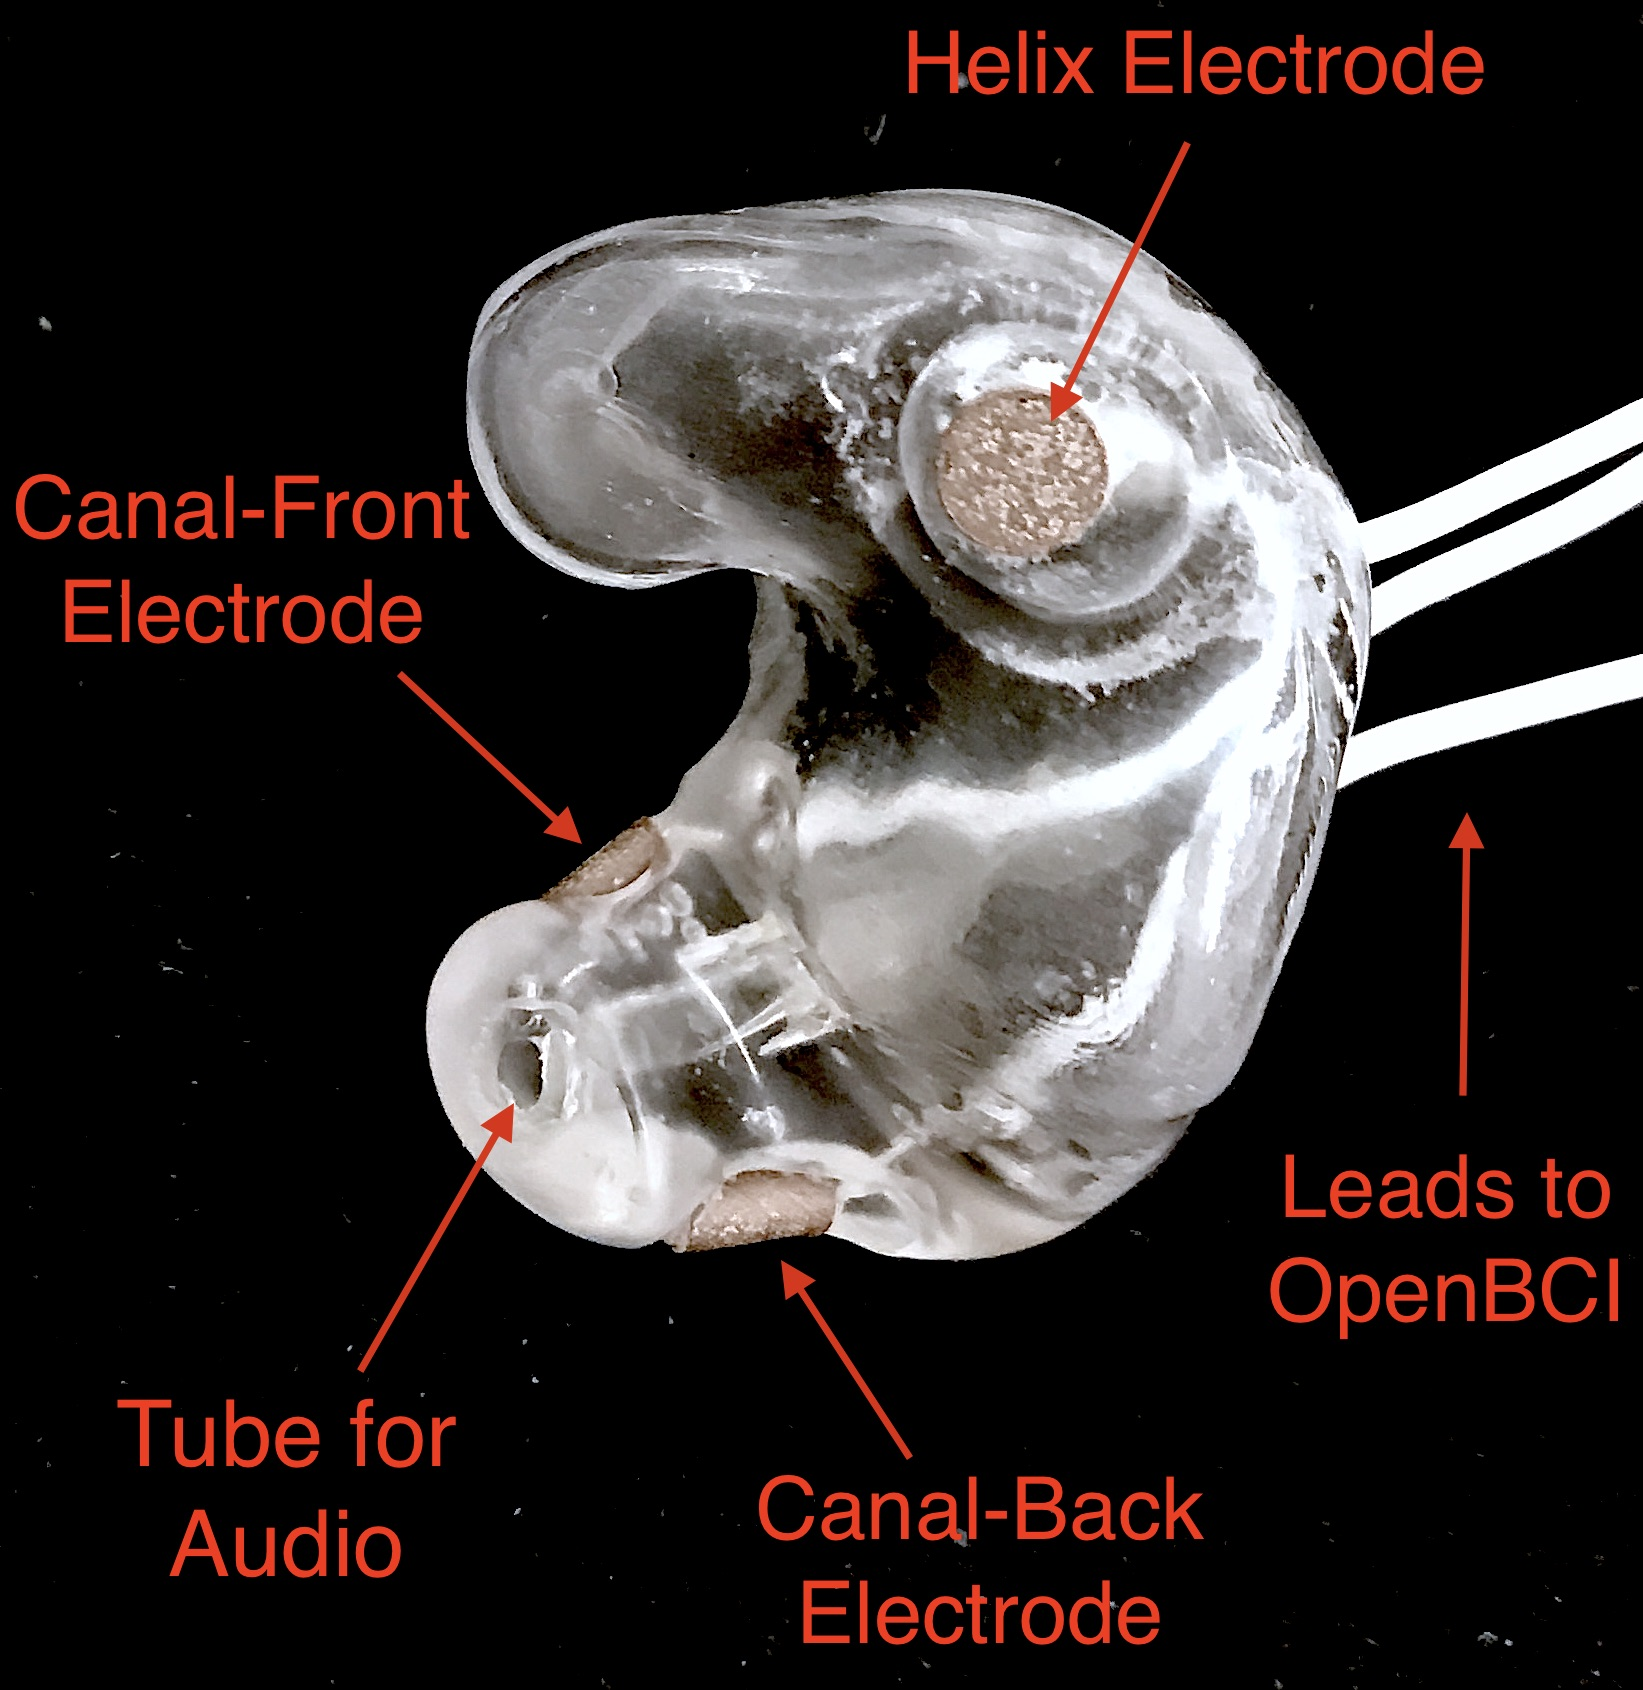
\includegraphics[width=.75\linewidth]{./figures/CFEEEG_piecefig_Right.jpg}
\caption{Labeled photo of one of our manufactured custom-fit earpieces with 3 embedded electrodes located in the concha, front-facing (anterior) in the ear canal, and back-facing (posterior) in the ear canal.}
\label{fig:earpiece_diagram}
\end{figure}

To produce custom ear impressions during the first study visit, we cleaned subjects' ears and injected silicon into the ear canals. A cotton ball with a string attached is placed into the ear canal first.  When the silicon dries after a few minutes, the string is pulled to remove the impression from the ear canal. This impression is then scanned with a 3D scanner and the resulting scan modified based on some heuristics to achieve a comfortable fit and to ensure the intended electrode sites will make good contact with the skin. Channels are created in the 3D model to allow wire leads and associated EEG electrodes as well as a plastic tube to deliver audio. This 3D model is then sent to a 3D printer. Following this wires, leads, and associated AgCl electrodes are installed. 

The positions of the earpiece electrodes were simplified from those described in \cite{Mikkelsen2015}. We reduced the number of canal electrodes in order to prevent electrical bridging and positioned them approximately 180 degrees apart in the canal (posterior/back and anterior/front locations in the canal). We also reduced the number of electrodes in the concha to one. An example of one of the manufactured earpieces is shown in Figure \ref{fig:earpiece_diagram}.

%\label{sec:orgaf30da9}
\subsection{Mental Tasks}

We used a set of mental tasks based on findings in related work regarding the relative strengths of different tasks in authentication accuracy and usability as reported by participants. Furthermore, given the in-ear placement of the electrodes and therefore the proximity to the temporal lobes containing the auditory cortex, we tested several novel authentication tasks based specifically on aural imagery or stimuli. The 9 authentication tasks and their attributes are listed in Table \ref{tab:tasks}. Our strategy was to select tasks that captured a diversity of possibilities across the dimensions of external stimuli, involving a personal secret, eyes open or closed (due to known significant effects on EEG), and different types of mental imagery.

\begin{table*}[t]
\centering
%% \begin{tabular}{llllll}
\begin{tabularx}{\textwidth}{llllll}

\textbf{Task} & \textbf{Description} & \textbf{Stimuli}? & \textbf{Secret}? & \textbf{Eyes} & \textbf{Imagery}\\
\hline
Breathe & Relaxed breathing with eyes closed & No & No & Closed & None\\
Breathe - Open & Relaxed breathing with eyes open & No & No & Open & None\\
Sport & Imagine attempting a chosen physical activity & No & Yes & Closed & Motor\\
Song & Imagine hearing a song & No & Yes & Closed & Aural\\
Song - Open & Song task, with eyes open & No & Yes & Open & Aural\\
Speech & Imagine a chosen spoken phrase & No & Yes & Closed & Aural\\
Listen & Listen to noise modulated at 40 Hz & Yes & No & Closed & None\\
Face & Imagine a chosen person's face & No & Yes & Closed & Visual\\
Sequence & Imagine a chosen face, number, and word on timed cues & Yes & Yes & Open & Visual\\
\hline
\end{tabularx}
\caption{Properties of authentication tasks. We selected tasks with a variety of different properties, but preferred tasks that did not require external stimuli, as the need to present such stimuli at authentication time could present challenges for usability and user security.}
\label{tab:tasks}%
\end{table*}

\subsection{Data Collection Protocol}
%\label{sec:org2041857}
All sites were cleaned with ethanol prior to electrode placement and a small amount of conductive gel was used on each electrode. For EEG recording we used OpenBCI \cite{michalska2009openbci}, an open-source biosensing system to maintain an overall low cost for our setup. OpenBCI costs about 600 USD, and thus is an affordable alternative to medical-grade EEG systems (about 20,000 USD), and has demonstrated effectiveness for non-medical use cases such as this one \cite{Frey2016}. The OpenBCI system we used allows for 8 channels of simultaneous recording, along with separate ground and reference channels. Data was collected with the ground placed at the center of the forehead, approximately AFz according to the 10-20 International Standard for Electrode Placement (ISEP), and using the left mastoid as reference. 6 channels were used for the three electrodes on Eech earpiece (shown in Figure \ref{fig:earpiece_diagram}), for the remaining two channels AgCl ring electrodes were placed on the right mastoid for later re-referencing, and at approximately Fp1 (above the left eye in in the ISEP) for validating the data collected in the ears against a common scalp-based placement. Before beginning the experiment, the data from each channel was visually inspected using the OpenBCI interface and participants were asked to blink and clench their jaws to confirm that all channels were active and properly connected. Audio stimuli were delivered through small tubes in the earpieces.

During the experiment, participants were seated in a comfortable position in a quiet room facing a laptop on which the instructions and stimuli were presented using PsychoPy \cite{peirce2007psychopy}. The entire set of tasks was completed once over with five trials each, followed by another five trials each in order to reduce boredom and repetition effects of a single task. Each trial was 10 seconds in length, for a total of 10 trials and 100 seconds of data collected per task. The instructions were read aloud to the participant by the experimenter, and the experiment was advanced using a pointer held in the participant's lap to minimize motion artifacts in the data. The experimenter also recorded the participant's chosen secrets for the \textit{sport}, \textit{song}, \textit{face}, \textit{speech}, and \textit{sequence} tasks and reminded the participant of these for the second set of trials.
 
 After completing the experiment, a subset of participants completed a usability questionnaire in which they were asked to rate their ease of performing, level of engagement, perceived repeatability, and likeliness of using each task. The questionnaire also asked participants to rank the tasks overall from most to least favorite, as well as several open response questions regarding potential use cases of in-ear EEG and this method of authentication, level of comfort wearing the earpieces, and any other comments they chose to provide.

\section{Analysis}
%\label{sec:org6c1a839}
\subsection{Data Validation}
%\label{sec:org800f2bd}

We were able to confirm the custom-fit earpieces are able to collect EEG data via two metrics: good impedances measured for the ear electrodes, and alpha-band EEG activity attenuation when a participant's eyes were open versus closed.

It is important that the electrical impedances achieved for electrodes are low ($<$10 kOhm) 
to obtain quality EEG signals. Table \ref{tab:impedances} below summarizes the impedances across the seven participants' six ear channels. With the exception of a few channels in select participants, impedances achieved were good overall. Most of the recorded impedances of the earpiece electrodes were less than 5 k\(\Omega\), a benchmark used widely in previous ear EEG work, and all except two were less than 10 k\(\Omega\). Nonetheless, the data from all electrodes were tested in the remaining two data quality tests.

\begin{table}[h]
\begin{center}
\begin{tabular}{lrrrrrr}
& \multicolumn{6}{c}{\textbf{Impedances} [k\(\Omega\)]} \\
\cline{2-7}
& \multicolumn{3}{|c|}{\textbf{Left ear}} & \multicolumn{3}{c|}{\textbf{Right ear}} \\
\textbf{P} & \textbf{C} & \textbf{F} & \textbf{B} & \textbf{C} & \textbf{F} & \textbf{B} \\
\hline
1 & 4 & 4 & 4 & \textless1 & 4 & 3\\
2 & 9 & 5 & 4 & 3 & 4 & 4\\
3 & 4 & 5 & 4 & 9 & 6 & 9\\
4 & 4 & 5 & 4 & 3 & 16 & 9\\
5 & 9 & 20 & 7 & 3 & 7 & 9\\
6 & 5 & 8 & 2 & 1 & 1 & 9\\
7 & 2 & 9 & 8 & 7 & 5 & 6\\
\end{tabular}
\end{center}
\caption{Electrical impedances measured for earpiece electrodes, for concha (C), front (F) and back (B).}
\label{tab:impedances}
\end{table}

For the alpha-attenuation test, data from the \textit{breathe} task was compared with that of the \textit{breathe - open} task. It is a well-known feature of EEG data that activity in the alpha-band (approximately 8-12 Hz range) increases when the eyes are closed compared with a similar state with eyes open. For our participants, this attenuation is clearly visible even in just a single trial's data. We also performed this comparison on the data collected from the Fp1 electrode and see the effect clearly there as well to compare. Figure \ref{fig:alpha_atten} shows the alpha attenuation in the left ear channels, as well as Fp1 of one participant as an example. We see the same effect in the right ear channels.

\begin{figure}[h]
\centering
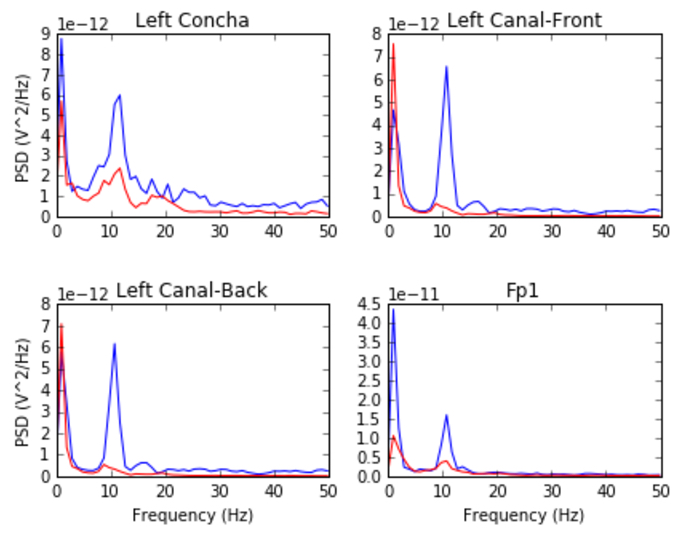
\includegraphics[width=0.5\textwidth]{figures/002_AlphaAtt_all.jpg}
\caption{Alpha-attenuation (8-12 Hz range) in left ear channels compared against the Fp1 channel, referenced at left mastoid. Red indicates breathing data with eyes open, blue indicates the same task with eyes closed.}
\label{fig:alpha_atten}
\end{figure}

\subsection{Classification}

We analyzed the EEG signals collected during the tasks using a support vector classifier (SVC). Since past work has shown that classification tasks in EEG-based BCI are linear \cite{Garrett2003a}, we used XGBoost, a popular tool for logistic linear classification \cite{Chen2016}. Compared to other linear classifiers, XGBoost uses gradient boosting; in which an algorithm generates an ensemble (in this case, a decision tree) of weak linear classifiers that minimizes a given loss function. Gradient boosting gives better results in linear classification problems, without our needing to manually tune classifier hyperparameter.

To produce feature vectors, we took slices of 100 raw values from each electrode (about 500ms of data), and performed a fourier transform to produce power spectra for each electrode during that slice. We concatenated all electrode power spectra together, and performed principal component analysis on all concatenated vectors such that the resulting vectors described 95\% of the variance in the full power spectrum data. For each task, for each participant, 100 seconds of data were collected in total across 10 trials of 10 seconds each, resulting in 200 samples per participant, per task, following this preprocessing.

We trained the classifier using a balanced sample of positive and negative examples, where positive examples were from the target participant and target task, and negative examples were randomly selected tasks from any participant besides the target participant. From this corpus of positive and negative samples, we withheld one third of data for testing. The remaining training set was fed into a XGBoost's cross-validation method, which we set to iteratively tweak parameters over a maximum of fifty rounds of cross-validation to minimize loss. After cross-validation, the updated classifier (with parameters applied) predicted labels on each sample in the test set, and we calculated FAR and FRR from its results.

\section{Results}
%\label{sec:org6705b1d}
\subsection{Combinations of electrodes}
%\label{sec:org21b14ae}

\begin{figure*}[t]
\centering
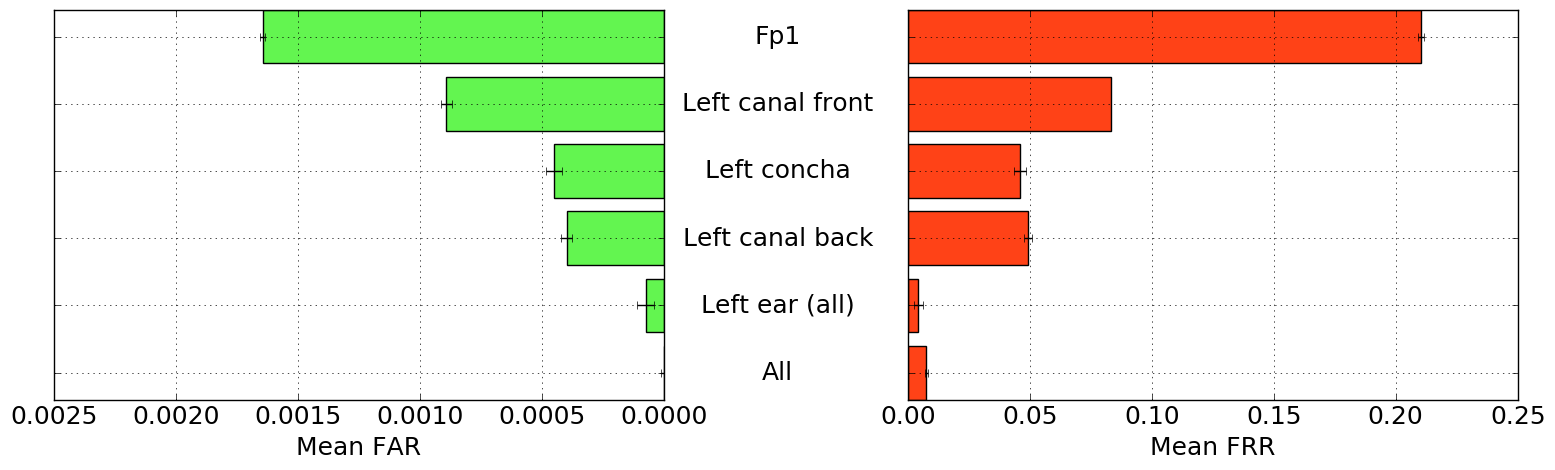
\includegraphics[width=.9\linewidth]{./figures/mean-far-and-frr-by-electrode-config.png}
\caption{FAR and FRR by electrode configuration. All electrodes (Fp1, right, and left ear channels) combined achieves a perfect FAR score. We achieve the next best scores using data from the left ear only.}
\label{fig:meanByElectrode}
\end{figure*}

For each configuration of electrodes, we calculated the mean FAR and FRR across all participants using each task as the passthought (Figure \ref{fig:meanByElectrode}).
Incorporating all electrodes data results in a perfect score for all tasks.
Using data from all left-ear electrodes achieves the next lowest FAR.
Interestingly, no single electrode performs as well as the aggregate left or both-ear plus Fp1 (all) conditions. 

Counter to our expectations, Fp1 does not perform as well as most ear electrodes, though overall these reported rates are far less than 1\%. 
For each position, FAR was about ten times lower than FRR, which is preferable for authentication, as false authentications are potentially more costly than false rejections.

Our results indicate acceptable accuracy using electrodes on the left ear alone. 
This corresponds to our original scenario, in which the device could be worn like an earbud (ideally, only one earbud would need sensors). As such, we focus on results from the left ear alone in our following analyses.

\subsection{Authentication Results}

In the previous section, we trained and tested a passthoughts classifier with each task as the passthought, for all participants. Our analyses revealed the left ear alone produced decent results. Using only data from the left ear electrodes, the performance of each task for each participant is shown in Table \ref{tab:farfrrall}. For each participant we find at least one task for which they achieve 0\% FAR and FRR, indicating perfect performance for this pool of users.

\begin{table*}[t]
\centering
\begin{tabularx}{.85\textwidth}{lrrrrrrrrrr}
& \multicolumn{2}{c}{\textbf{P1}} & \multicolumn{2}{c}{\textbf{P2}} & \multicolumn{2}{c}{\textbf{P3}} & \multicolumn{2}{c}{\textbf{P5}} & \multicolumn{2}{c}{\textbf{P7}}\\
\textbf{Task} & FAR & FRR & FAR & FRR & FAR & FRR & FAR & FRR & FAR & FRR\\ \hline
Breathe & 0.0002 & 0 & 0 & 0 & 0 & 0 & 0 & 0.0127 & 0 & 0\\
Breathe - open & 0.0002 & 0.0127 & 0 & 0 & 0 & 0 & 0 & 0.0253 & 0 & 0\\
Face & 0.0002 & 0.0253 & 0.0005 & 0.0253 & 0 & 0.0127 & 0 & 0 & 0 & 0\\
Listen & 0 & 0 & 0.0005 & 0 & 0 & 0 & 0 & 0 & 0 & 0\\
Sequence & 0 & 0.0506 & 0.0002 & 0 & 0 & 0 & 0 & 0 & 0.0007 & 0.0127\\
Song	 & 0.0002 & 0.0380 & 0 & 0 & 0	 & 0 & 0 & 0.0127 & 0.0007 & 0.0127\\
Song - open & 0.0002 & 0.0127 & 0 & 0 & 0 & 0 & 0 & 0 & 0 & 0.0127\\
Speech & 0.0002 & 0 & 0.0005 & 0 & 0 & 0 & 0 & 0 & 0 & 0\\
Sport & 0.0002 & 0 & 0 & 0 & 0 & 0 & 0 & 0  & 0 & 0.0127\\
\textbf{Best Task} & 0 & 0 & 0 & 0 & 0 & 0 & 0 & 0 & 0 & 0\\ \hline
\end{tabularx}
\caption{FAR and FRR performance of each task for each participant using data from the left ear. P4 and P6 achieve perfect zero FARs and FRRs across all tasks and so are not shown here.}
\label{tab:farfrrall}
\end{table*}

All best-performing tasks in our best-case set achieved perfect FAR and FRRs. Interestingly, \textit{breathe} appeared as the best task across all participants, except P1 whose best task was \textit{listen} and P5 who had several other best performing tasks. Given our training strategy, these results indicate that a given person's \textit{breathe} task is distinguishable not only among other tasks, but among \textit{breathe} tasks from other participants.
This task performed about as well as its open-eyes counterpart (Figure \ref{fig:meanByTask}), as did \textit{song - open} and \textit{sport} (though, interestingly, \textit{song} with eyes closed performed less well).

\begin{figure*}[t]
\centering
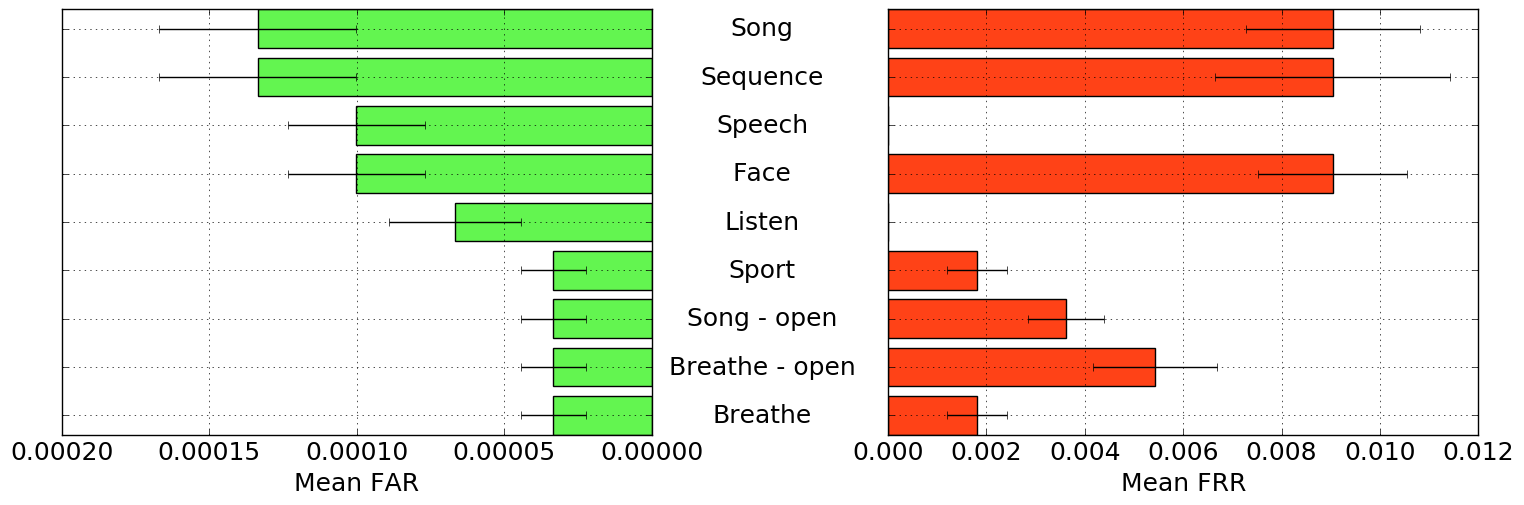
\includegraphics[width=.9\linewidth]{./figures/mean-far-and-frr-by-task.png}
\caption{FAR and FRR results by task, across all subjects, using data from the left ear only.}
\label{fig:meanByTask}
\end{figure*}

These results establish good performance in our original training strategy, in which we count as negative examples recordings from the wrong participant performing any task. For comparison, we try two additional training strategies: one in which negative examples are the correct task recorded from the wrong participant (within-tasks), and one in which negative examples are the incorrect task recorded from the correct participant (within-participants).

\begin{table}[h]
\begin{center}
\begin{tabular}{lrr}
 & \textbf{FAR} & \textbf{FRR}\\
\hline
Original & 0.000074 & 0.004424\\
Within-tasks & 0.000724 & 0.001522\\
Within-participants & 0.002523 & 0.039702\\
\hline
\end{tabular}
\end{center}
\caption{Mean FAR and FRR for all participants and passthoughts across three different training strategies.}
\label{tab:compare}
\end{table}

Overall, our original training strategy achieves the lowest FAR (Table \ref{tab:compare}). Within-tasks FAR is ten times higher, and within-participants FAR is one hundred times higher, though for all scenarios still less than 1\%.
However, FRR is \textit{lower} in the within-tasks training strategy than in our original strategy's FRR. Within-participants again results in the highest FRR.

\subsection{Usability}

A subset of four participants completed our usability questionnaire. This questionnaire asked them to rank each of the mental tasks on 7-point likert-type scales on ease of use, level of engagement, perceived repeatability, and likeliness to use in a real-world authentication setting. The \textit{breathe} and \textit{listen} (\(\mu\)=6.75) tasks were rated easiest to use. \textit{Sequence} (\(\mu\)=5) and \textit{song} were rated highest in engagement, \textit{Breathe} (\(\mu\)=7) and \textit{listen} (\(\mu\)=6.75) were ranted highest in repeatability. In terms of likeliness of use for authentication, \textit{song-open} (\(\mu\)=5) and \textit{sequence} (\(\mu\)=4.25) were rated highest, though modestly. We also asked participants to rank the tasks from most (1) to least (9) favorite overall. The \textit{song - open} task ranked highest among favorites (\(\mu\)=4.25) followed by a tie between \textit{breathe - open}, \textit{song}, and \textit{speech} (\(\mu\)=4.75). \textit{Sequence} (\(\mu\)=7.75) and \textit{face} (\(\mu\)=6.75) were rated as least favorites.

In addition to the scales and rankings, we included in our questionnaire a few open response questions to ascertain attitudes about the use cases for in-ear EEG and passthoughts, and the comfort of wearing an in-ear EEG device in everyday life. Participants first read the prompt, "Imagine a commercially available wireless earbud product is now available based on this technology that you've just experienced. It requires minimal effort for you to put on and wear.", and were asked about use cases for in-ear EEG and passthoughts. Responses about in-ear EEG expectedly included authentication for unlocking a phone or computer and building access, but also aspects of self-improvement such as P4's response "Help people increase focus and productivity". P5 and P6 also indicated a use for measuring engagement with media like movies and music, and relatedly P4 wrote "music playback optimized for current mental state and feelings". In terms of comfort wearing such a device, participants generally responded they would be comfortable, though P5 and P6 stipulated only when they would otherwise be wearing something like earphones in their ears already. In response to an "any other comments" prompt, notably three participants pointed out the mental imagery of a face was difficult for them and some concerns about their ability to repeat tasks in the same exact way each time.

A final component of usability we acquired was the ability of the participants to recall their specific chosen passthoughts for the \textit{song}, \textit{sport}, \textit{speech}, \textit{face}, and \textit{sequence} tasks. Participants were contacted approximately two weeks after their data collection study visit and were prompted with these categories and asked to respond with what they chose during the experiment. All participants were able to recall all of their chosen secrets, with the exception of one participant who incorrectly remembered their chosen word for the \textit{sequence} task. 

\section{Imposter Attack}

While our authentication analysis establishes that passthoughts achieve low FAR and FRR when tested against other participants' passthoughts, we do not know how robust passthoughts are against a spoofing attack, in which both a participant's custom-fit electrode, and details of that participant's chosen passthought, are leaked and used by an imposter. 

The first aspect of this scenario we tested was the ability of an imposter to wear an earpiece acquired from someone else and achieve viable impedance values for EEG collection based on the fit of the pieces in their ears. P1 tried on each of the other participants' earpieces, which were able to at least physically fit in P1's ears. The impedances of P1 wearing other participants' earpieces were then recorded and are listed in Table \ref{tab:imposter_impedances} below. While some are a better fit than others, overall they are higher than those achieved by the pieces' intended owners themselves.

\begin{table}[h]
\begin{center}
\begin{tabular}{lrrrrrr}
& \multicolumn{6}{c}{Impedances [k\(\Omega\)]} \\
\cline{2-7}
& \multicolumn{3}{|c|}{\textbf{Left ear}} & \multicolumn{3}{c|}{\textbf{Right ear}} \\
\textbf{P} & \textbf{C} & \textbf{F} & \textbf{B} & \textbf{C} & \textbf{F} & \textbf{B} \\
\hline
2 & 34.1 & 10.2 & 12.8 & 27.8 & 16.0 & 16.3\\
3 & 21.1 & 20.9 & 19.0 & 13.5 & 11.3 & 19.5\\
4 & 14.1 & 11.9 & 9.7 & 11.0 & 11.1 & 13.3\\
5 & 17.2 & 21.9 & 10.3 & 32.6 & 12.5 & 11.6\\
6 & 18.7 & 10.0 & 8.4 & 14.8 & 11.5 & 8.9\\
7 & 91.5 & \textgreater1000 & 21.5 & 33.5 & 26.4 & 31.0\\
\end{tabular}
\end{center}
\caption{Electrical impedances achieved with P1 wearing each other participant's (P) custom-fitted earpieces, for concha (C), front (F) and back (B).}
\label{tab:imposter_impedances}
\end{table}

To explore the scenario of an imposter attempting to gain access, we chose the most vulnerable case participant, P6, whose earpieces P1 had the lowest impedances while wearing. We collected data using the same data collection protocol, but had P1 refer to P6's report of chosen passsthoughts.
P1 performed each of P6's passthoughts (simulating an "inside imposter"). Following the same classification and preprocessing steps, we generated 200 samples per task for our imposters, using data from all left ear electrodes.

% \begin{table}[h]
% \begin{center}
% \begin{tabular}{lll}
% Task & FAR (Insider) & FAR (Outsider)\\
% \hline
% Breathe & 0.0 & 0.0\\
% Breathe - Open & 0.0 & 0.0\\
% Sport & 0.0 & 0.0\\
% Song & 0.0 & 0.0\\
% Song - Open & 0.0 & 0.0\\
% Speech & 0.0 & 0.0\\
% Listen & 0.0 & 0.0\\
% Face & 0.0 & 0.0\\
% Sequence & 0.0 & 0.0\\
% \end{tabular}
% \end{center}
% \caption{False acceptance rate for spoofed versions of P6's passthoughts, performed by an inside imposter (P1 from the original participant pool) and an outside imposter (not from the original participant pool).}
% \label{tab:imposter}
% \end{table}

Since every participant has one classifier per task (for which that task is the passthought), we are able to make 200 spoofed attempts with the correct passthought on each of P6's classifiers. We find no successful spoof attempts for tasks with a chosen secret (e.g., \textit{song} or \textit{face}). However, we also do not find any successful spoof attacks for tasks with no chosen secret (e.g., \textit{breathe}). In fact, in all 1,800 spoof attempts (200 attempts for each of the 9 classifiers), we do not find a single successful attack on any of P6's classifiers.

However, since this participant's data appeared in the initial pool, the classifier may have been trained on his or her recordings as negative examples. To explore the efficacy of an outsider spoofing recordings, we repeated the same protocol with an individual who did not appear in our initial set of participants (an "outside imposter"). Again, we find zero successful authentication attempts out of 1,800 attempts.

\section{Discussion}

Our findings demonstrate the apparent feasibility of a single earpiece, achieving good results with only three electrodes and a reference, all on or around the left ear. FARs and FRRs are very low across all participants and tasks, with FARs overall lower than FRRs, a desirable pattern in terms of authenticating access to potentially sensitive information. Participants' best-performing passthoughts typically see no errors in our training. Furthermore, no spoofed attacks were successful in our cursory analysis.

This study was conducted with a small, relatively homogeneous sample of participants. In order to establish the validity of this system for widespread real-world use we feel it is necessary to expand the size and diversity of participants in future studies. In the case of this initial evaluation however, the homogeneity of our participant pool strengthens the reported results given that system attempts to distinguish between individuals. We feel that a greater number of  participants from a more diverse pool would greatly improve our understanding and interpretation of the capabilities of this technology. This sample size is in line with this area of research as it is comparable to that of other scalp-based EEG passthoughts work\cite{Ashby2011, Marcel2007a, Palaniappan2008, palaniappan2006electroencephalogram, Poulos2002, Chuang2013b}, the only other in-ear EEG passthoughts study we are aware of \cite{curran2016passthoughts} (notably a generic fit system was used here), and other custom-fit in-ear EEG research \cite{Kidmose2013a}. The fitting and manufacturing of custom-fit earpieces was the main limitation to increasing our sample size, and may very well pose a limitation in proliferation and adoption of such a technology in the world. Recently, there have been developments in at-home kits for creating one's own custom-fitted earpieces \cite{voix2015settable} that could help overcome this barrier.

In our analysis, some notable patterns emerged. First, the \textit{breathe},
\textit{breathe-open}, and \textit{listen} tasks performed exceedingly well among participants.
Classifiers overall distinguished the \textit{breathe}  and \textit{listen} tasks even compared
to the same tasks from other participants, implying that these tasks are expressed differently
for each participant, i.e. that they have an inherence factor sufficient for authentication,
even though they task do not involve an explicit secondary knowledge factor as in \textit{sport}
or \textit{song}, for example. Second, we were able to achieve good results by generating feature
vectors based on only 500ms (300 voltage readings across the three electrodes).
This short timespan is somewhat surprising, given that some tasks (like songs)
presumably rely on changes or patterns over a longer period of time.

Furthermore, low impedances are still achievable by an imposter using other participants' custom-fit earpieces, despite the uniqueness of ear canal shapes between individuals \cite{Akkermans2005} likely in part due to the our of conductive gel. This discovery is not detrimental, however, as the inherence factor of this system is drawn from the uniqueness of EEG and not ear canal shape. Classifiers appear to still resists spoofing attacks, indicating that task-related signals are unique to individuals. In terms of establishing a possession factor, the custom-fit earpieces could easily include a hardware keypair to sign authentication attempts in a three-factor, one-step scheme.

The powerful interactions between inherence and knowledge emerged in our spoofing attack. Although our target participant documented their chosen passthought, the spoofers found ambiguity in how these passthoughts could be expressed. For the \textit{face} task, the spoofers did not know the precise face the original participant had chosen. For the \textit{song} and \textit{song - open} tasks, though the song was known, the spoofers did not know what part of the song the original participant had imagined, or how it was imagined (humming, imagining a full performance, melody, vocals, etc). This experience sheds light on the highly individual nature of passthoughts, and provides a positive indication that there may be some intrinsic difficulty in spoofing attempts of passthoughts.

Finally, performance on Fp1 was not as high as performance in the ear, despite Fp1's popularity in past work on passthoughts \cite{Chuang2013b}. This could be explained by the greater number of electrodes in the ear in this analysis (compared to just one on Fp1). Additionally, Fp1 is best poised to pick up on frontal lobe activity (e..g, concentration), but our tasks did not generally involve frontal lobe activity; in fact, a good number of them involved audio, which we would expect to be better observed from the auditory cortex near the ears. Future work should continue to investigate what sorts of mental tasks best lend themselves to in-ear recording.

\section{Future Work}

One primary question surrounds how our passthoughts system performance will change with a greater number of users, and with more diverse data. Our system specifically trains on negative examples of incorrect users; we do not yet know how this approach will scale. At the same time, we must investigate the stability of EEG readings for a passthought over time to establish long-term usability. We must also collect EEG data from the variety of different user states: ambulatory settings, during physical exertion or exercise, under the influence of caffeine or alcohol, etc.

% We provide cursory evidence that passthoughts are difficult to spoof, though further work should expand on ours with more subjects.
Another important question surrounds how passthoughts might be cracked. Generally, we do not understand how an individual's passthought is drawn from the distribution of EEG signals that an individual produces throughout the day. Given a large enough corpus of EEG data, are some passthoughts as easy to guess as \textit{password1234} is for passwords? Future work should perform statistical analysis on passthoughts, such as clustering (perhaps with t-SNE) to better understand the space of possible passthoughts. This work will allow us simulate cracking attempts, and to develop empirically motivated strategies for prevention, e.g., locking users out after a certain number of attempts. This work could also reveal interesting tradeoffs between the usability or accuracy of passthoughts and their security.

Finally, our work leaves room for some clear user experience (UX) improvements.
Future work should try using dry electrodes, commonly found in consumer EEG devices, for comfort and usability. The electrodes could be grounded to the ear, instead of the forehead. Additionally, future work could easily place a speaker inside our current custom-fit earbuds to produce working "hearables'' that can be used as ordinary headphones.

Future work should also attempt a closed-loop (or online) passthought system, in which users receive immediate feedback on the result of their authentication attempt. A closed-loop BCI system could help us understand how learning effects on the human side might impact authentication performance, as the human and machine co-adapt through authentication attempts.

\section{Conclusion}

As demonstrated by these preliminary results, custom-fit, in-ear EEG earpieces provide three factors of authentication in one highly usable authentication step: thinking one's passthought, using the discreet form factor of an earpiece. In this paper, we demonstrate quite high authentication accuracy using a single sensing earpiece with potential for integration with technology already used in everyday life like earphones. By expanding our corpus of EEG readings (in population size, time, and diversity of settings), we hope to better understand the underlying distribution of EEG signals and security properties of passthoughts as well usability issues that may arise in different contexts.

\section{Acknowledgments}

This work was funded by X.

% Balancing columns in a ref list is a bit of a pain because you
% either use a hack like flushend or balance, or manually insert
% a column break.  http://www.tex.ac.uk/cgi-bin/texfaq2html?label=balance
% multicols doesn't work because we're already in two-column mode,
% and flushend isn't awesome, so I choose balance.  See this
% for more info: http://cs.brown.edu/system/software/latex/doc/balance.pdf
%
% Note that in a perfect world balance wants to be in the first
% column of the last page.
%
% If balance doesn't work for you, you can remove that and
% hard-code a column break into the bbl file right before you
% submit:
%
% http://stackoverflow.com/questions/2149854/how-to-manually-equalize-columns-
% in-an-ieee-paper-if-using-bibtex
%
% Or, just remove \balance and give up on balancing the last page.
%
%\balance

% REFERENCES FORMAT
% References must be the same font size as other body text.

\bibliographystyle{acm-sigchi}
\bibliography{references.bib}

\end{document}